\documentclass[handout]{beamer}
\usepackage[T1]{fontenc}
\usepackage[english]{babel}
\usefonttheme{serif}
\setbeamertemplate{navigation symbols}{
\usebeamerfont{footline}
\usebeamercolor[fg]{footline}
\insertframenumber/\inserttotalframenumber{}
}
\setbeamerfont{frametitle}{size = \small}
\usepackage{mathpazo}
\usepackage{float}
\usepackage[labelsep = colon]{caption}
\usepackage{amsmath}
\usepackage{setspace}
\usepackage{graphicx}
\usepackage{threeparttablex}
\usepackage{longtable}
\usepackage{booktabs}
\usepackage{dcolumn}
\usepackage{pdfpages}
\usepackage{ulem}


\title{GV217 Conflict Analysis, Week 22}
\subtitle{Gender and Conflict}
\author{Muzhou Zhang\\ muzhou.zhang@essex.ac.uk\\ Virtual Office Hour: 15:30--16:30, Friday, 997 5800 8679}
\date{04 Mar 2022}

\begin{document}
\maketitle
\setstretch{1.25}

\begin{frame}{Women in Conflicts: Cases}
    \pause
    Customary evil
    \begin{tabular}{ll}
        Conflict                                                    & Estimated rapes \\
        Second Sino-Japanese war, Nanking, 1937                     & 20,000          \\
        Soviet army in Germany, WWII                                & 100,000--2m     \\
        The Bangladesh war of secession, 1971                       & 200,000         \\
        Bosnian war, 1992--95                                       & 20,000          \\
        Sierra Leone civil war, 1991--2002                          & Over 50,000     \\
        Rwandan genocide, 1994                                      & 500,000        
    \end{tabular}
    \tiny \emph{The Economist}, \url{https://www.economist.com/international/2011/01/13/wars-overlooked-victims}
\end{frame}

\begin{frame}{Women in Conflicts: Cases}
    \pause
    \begin{center}
        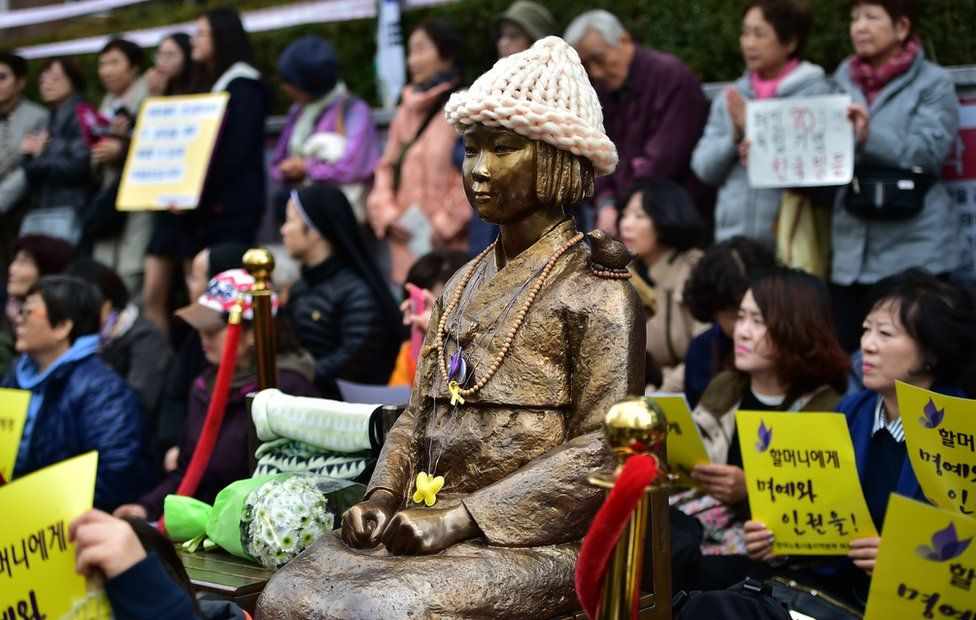
\includegraphics[width = \linewidth]{/Users/mz/Desktop/GitHub/teaching/gv217_conflict_analysis/figs/wk22/fig1.png}
    \end{center}
    \tiny © AFP, \url{https://www.bbc.co.uk/news/world-asia-35190464}
\end{frame}

\begin{frame}{Women in Conflicts: Cases}
    \pause
    \begin{center}
        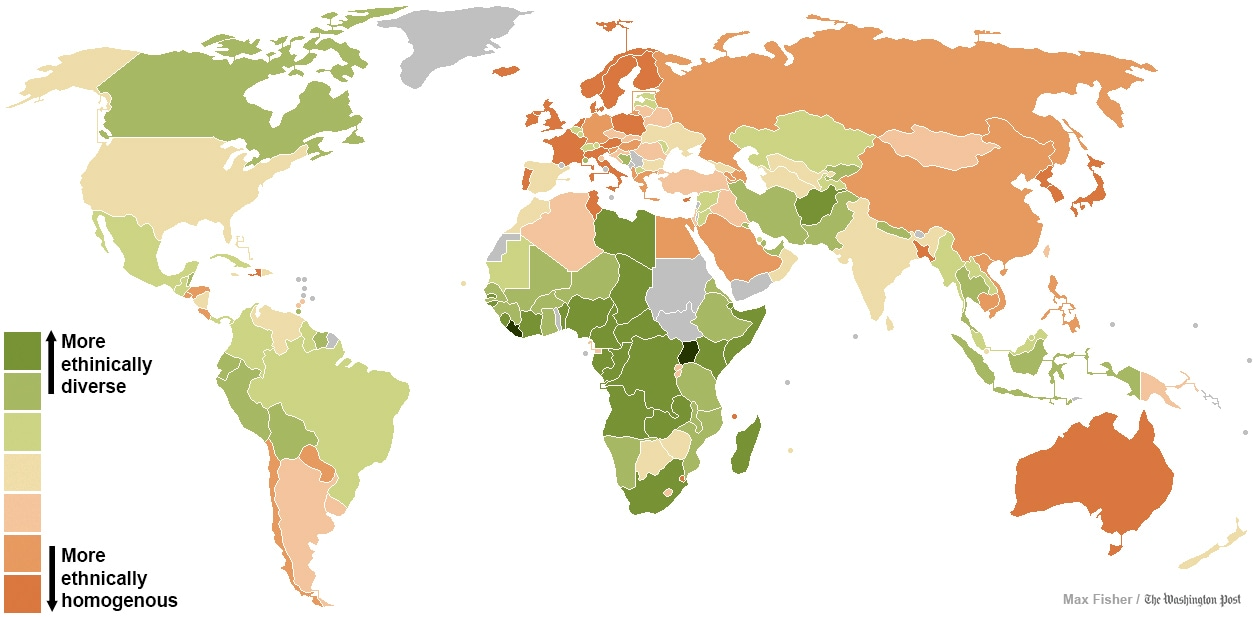
\includegraphics[width = \linewidth]{/Users/mz/Desktop/GitHub/teaching/gv217_conflict_analysis/figs/wk22/fig2.png}
    \end{center}
\end{frame}

\begin{frame}{Women in Conflicts: Cases}
    \pause
    \begin{center}
        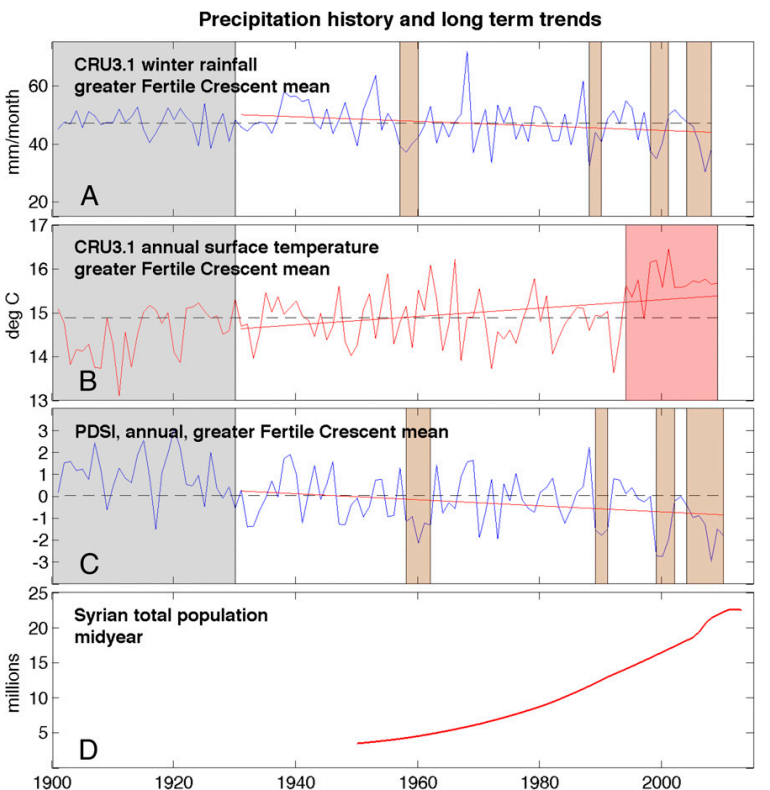
\includegraphics[width = \linewidth]{/Users/mz/Desktop/GitHub/teaching/gv217_conflict_analysis/figs/wk22/fig3.png}
    \end{center}
\end{frame}

\begin{frame}{Women in Conflicts: Cases}
    \pause
    \begin{center}
        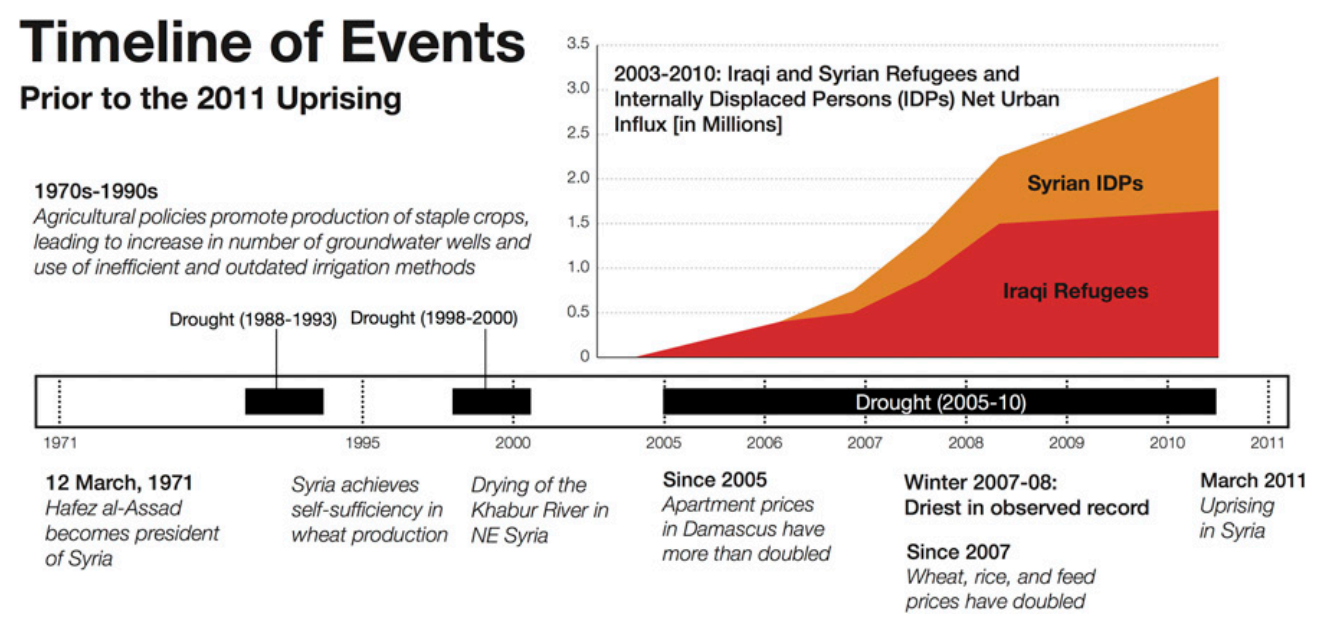
\includegraphics[width = \linewidth]{/Users/mz/Desktop/GitHub/teaching/gv217_conflict_analysis/figs/wk22/fig4.png}
    \end{center}
\end{frame}

\begin{frame}{Women in Conflicts: Cases}
    \pause
    \begin{center}
        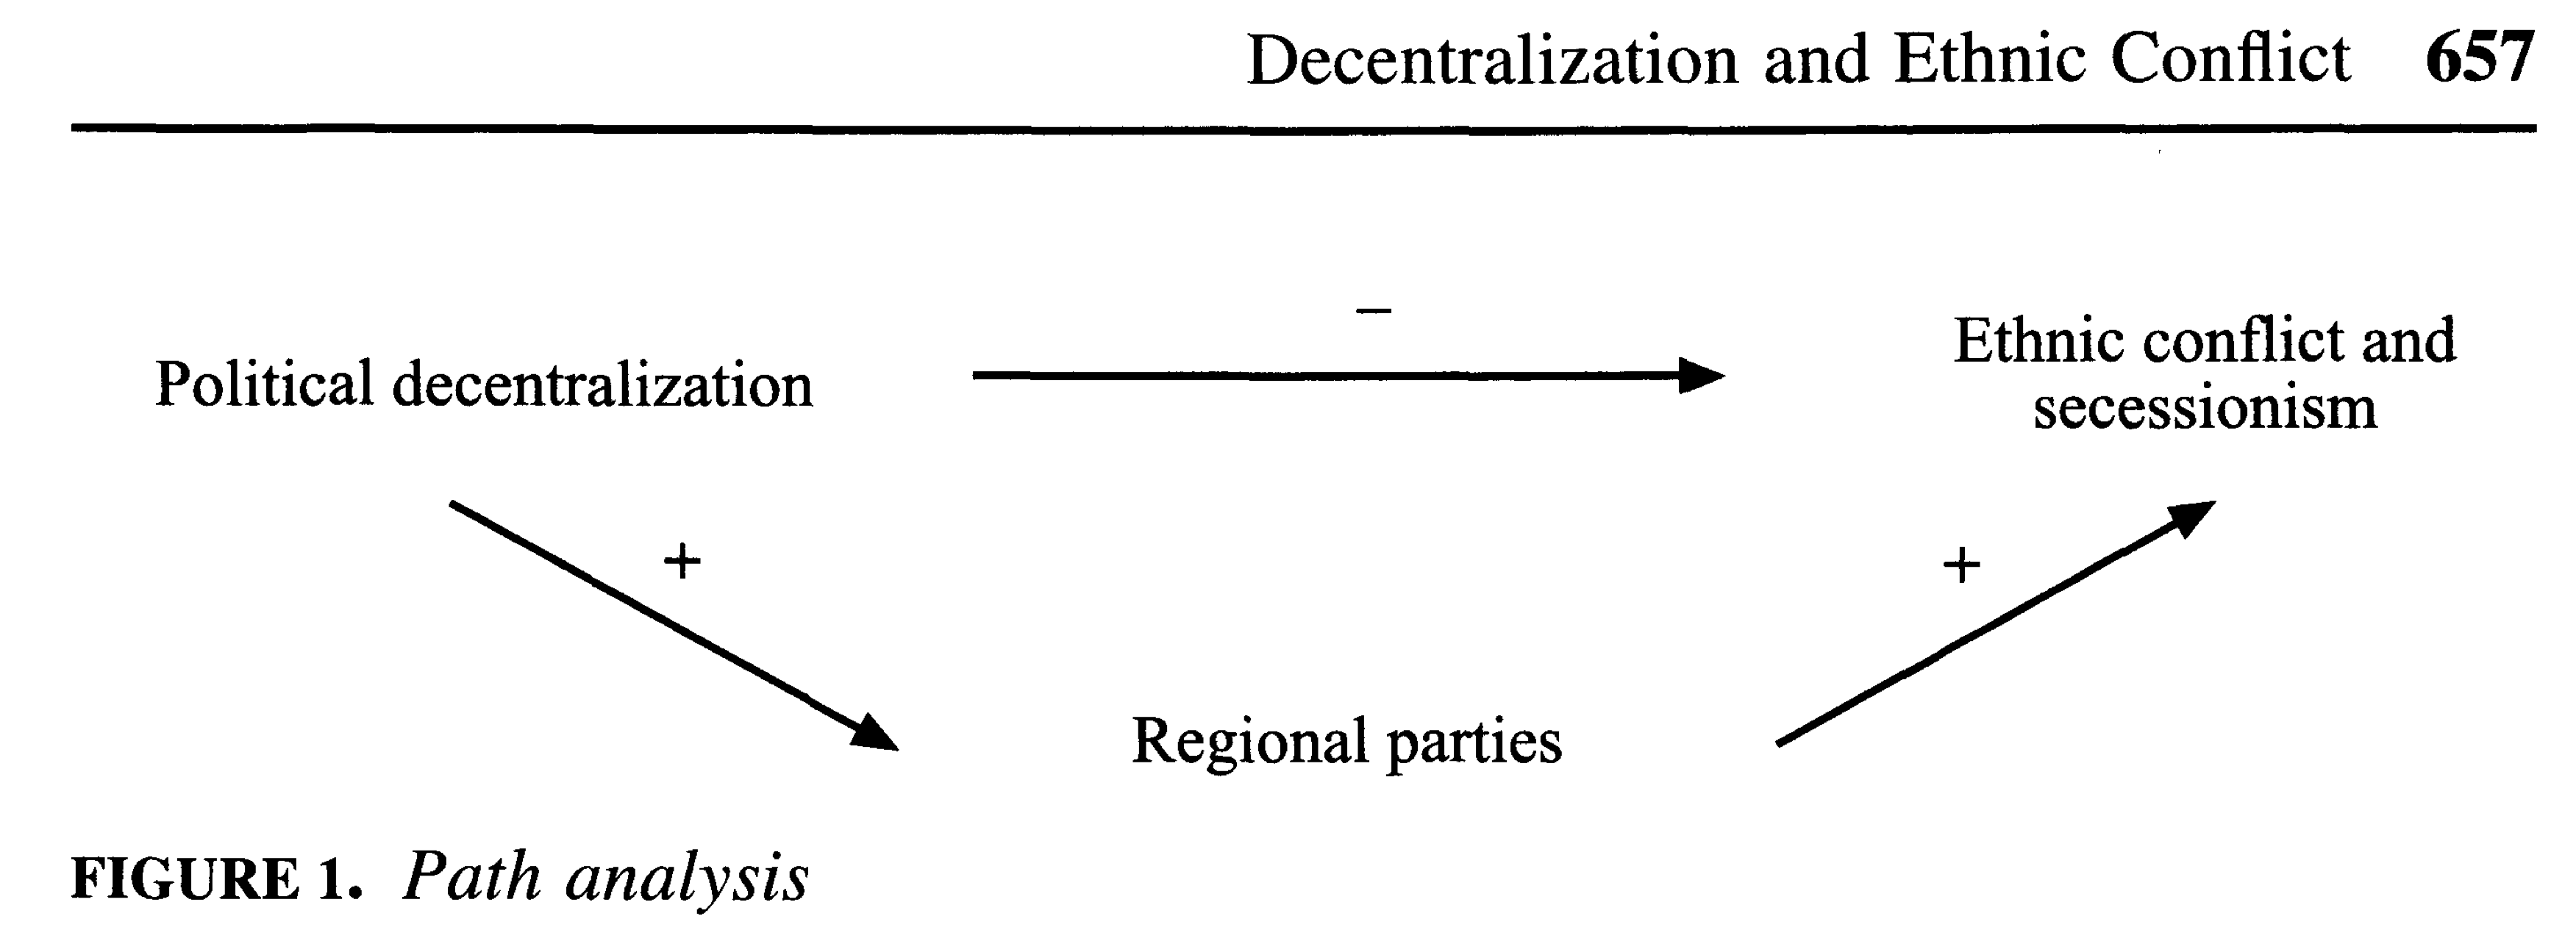
\includegraphics[width = \linewidth]{/Users/mz/Desktop/GitHub/teaching/gv217_conflict_analysis/figs/wk22/fig5.png}
    \end{center}
    \tiny © GETTY IMAGES, \url{https://www.bbc.co.uk/news/world-africa-57187736}
\end{frame}

\begin{frame}{Women in Conflicts: Cases}
    \pause
    \begin{center}
        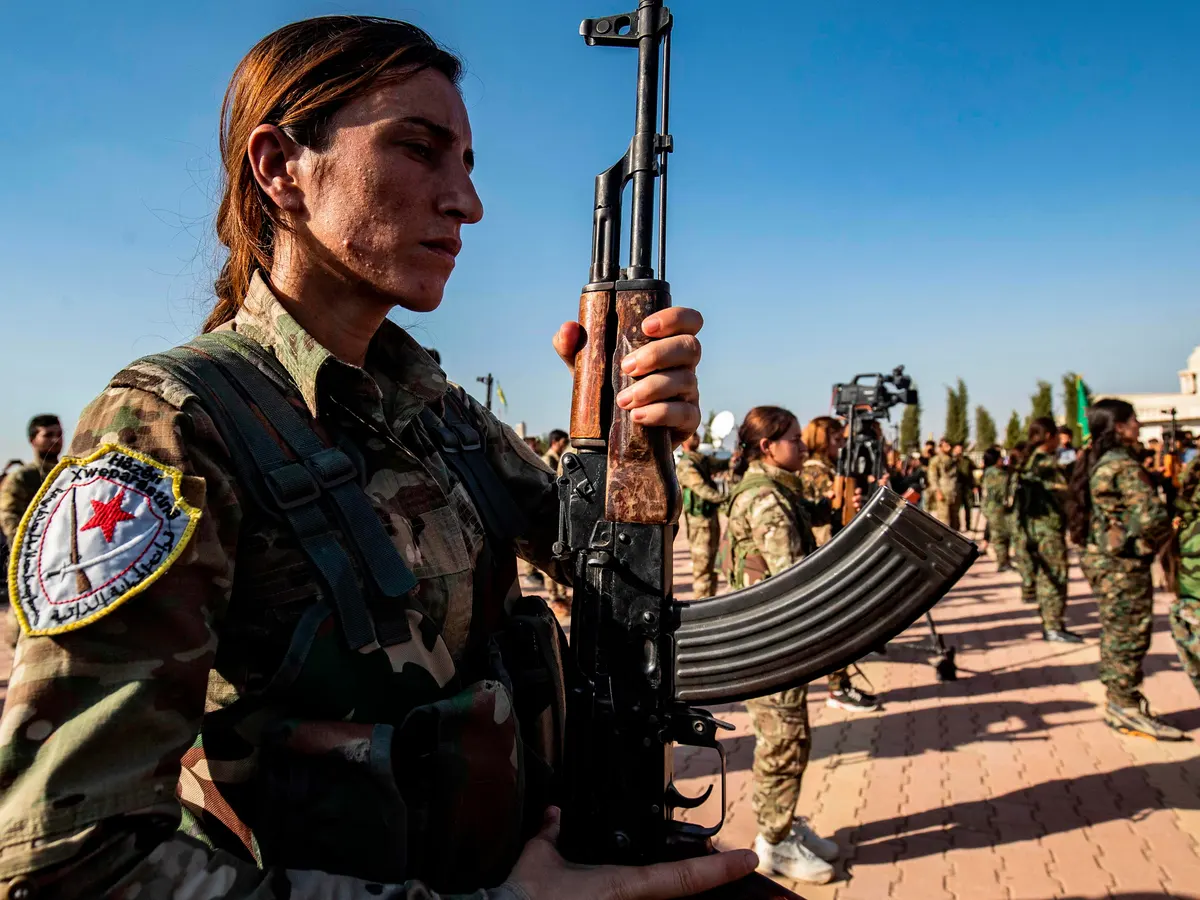
\includegraphics[width = \linewidth]{/Users/mz/Desktop/GitHub/teaching/gv217_conflict_analysis/figs/wk22/fig6.png}
    \end{center}
    \tiny Delil Souleiman/AFP via Getty Images
\end{frame}

\begin{frame}{Women in Conflicts: Cases}
    \pause
    \begin{center}
        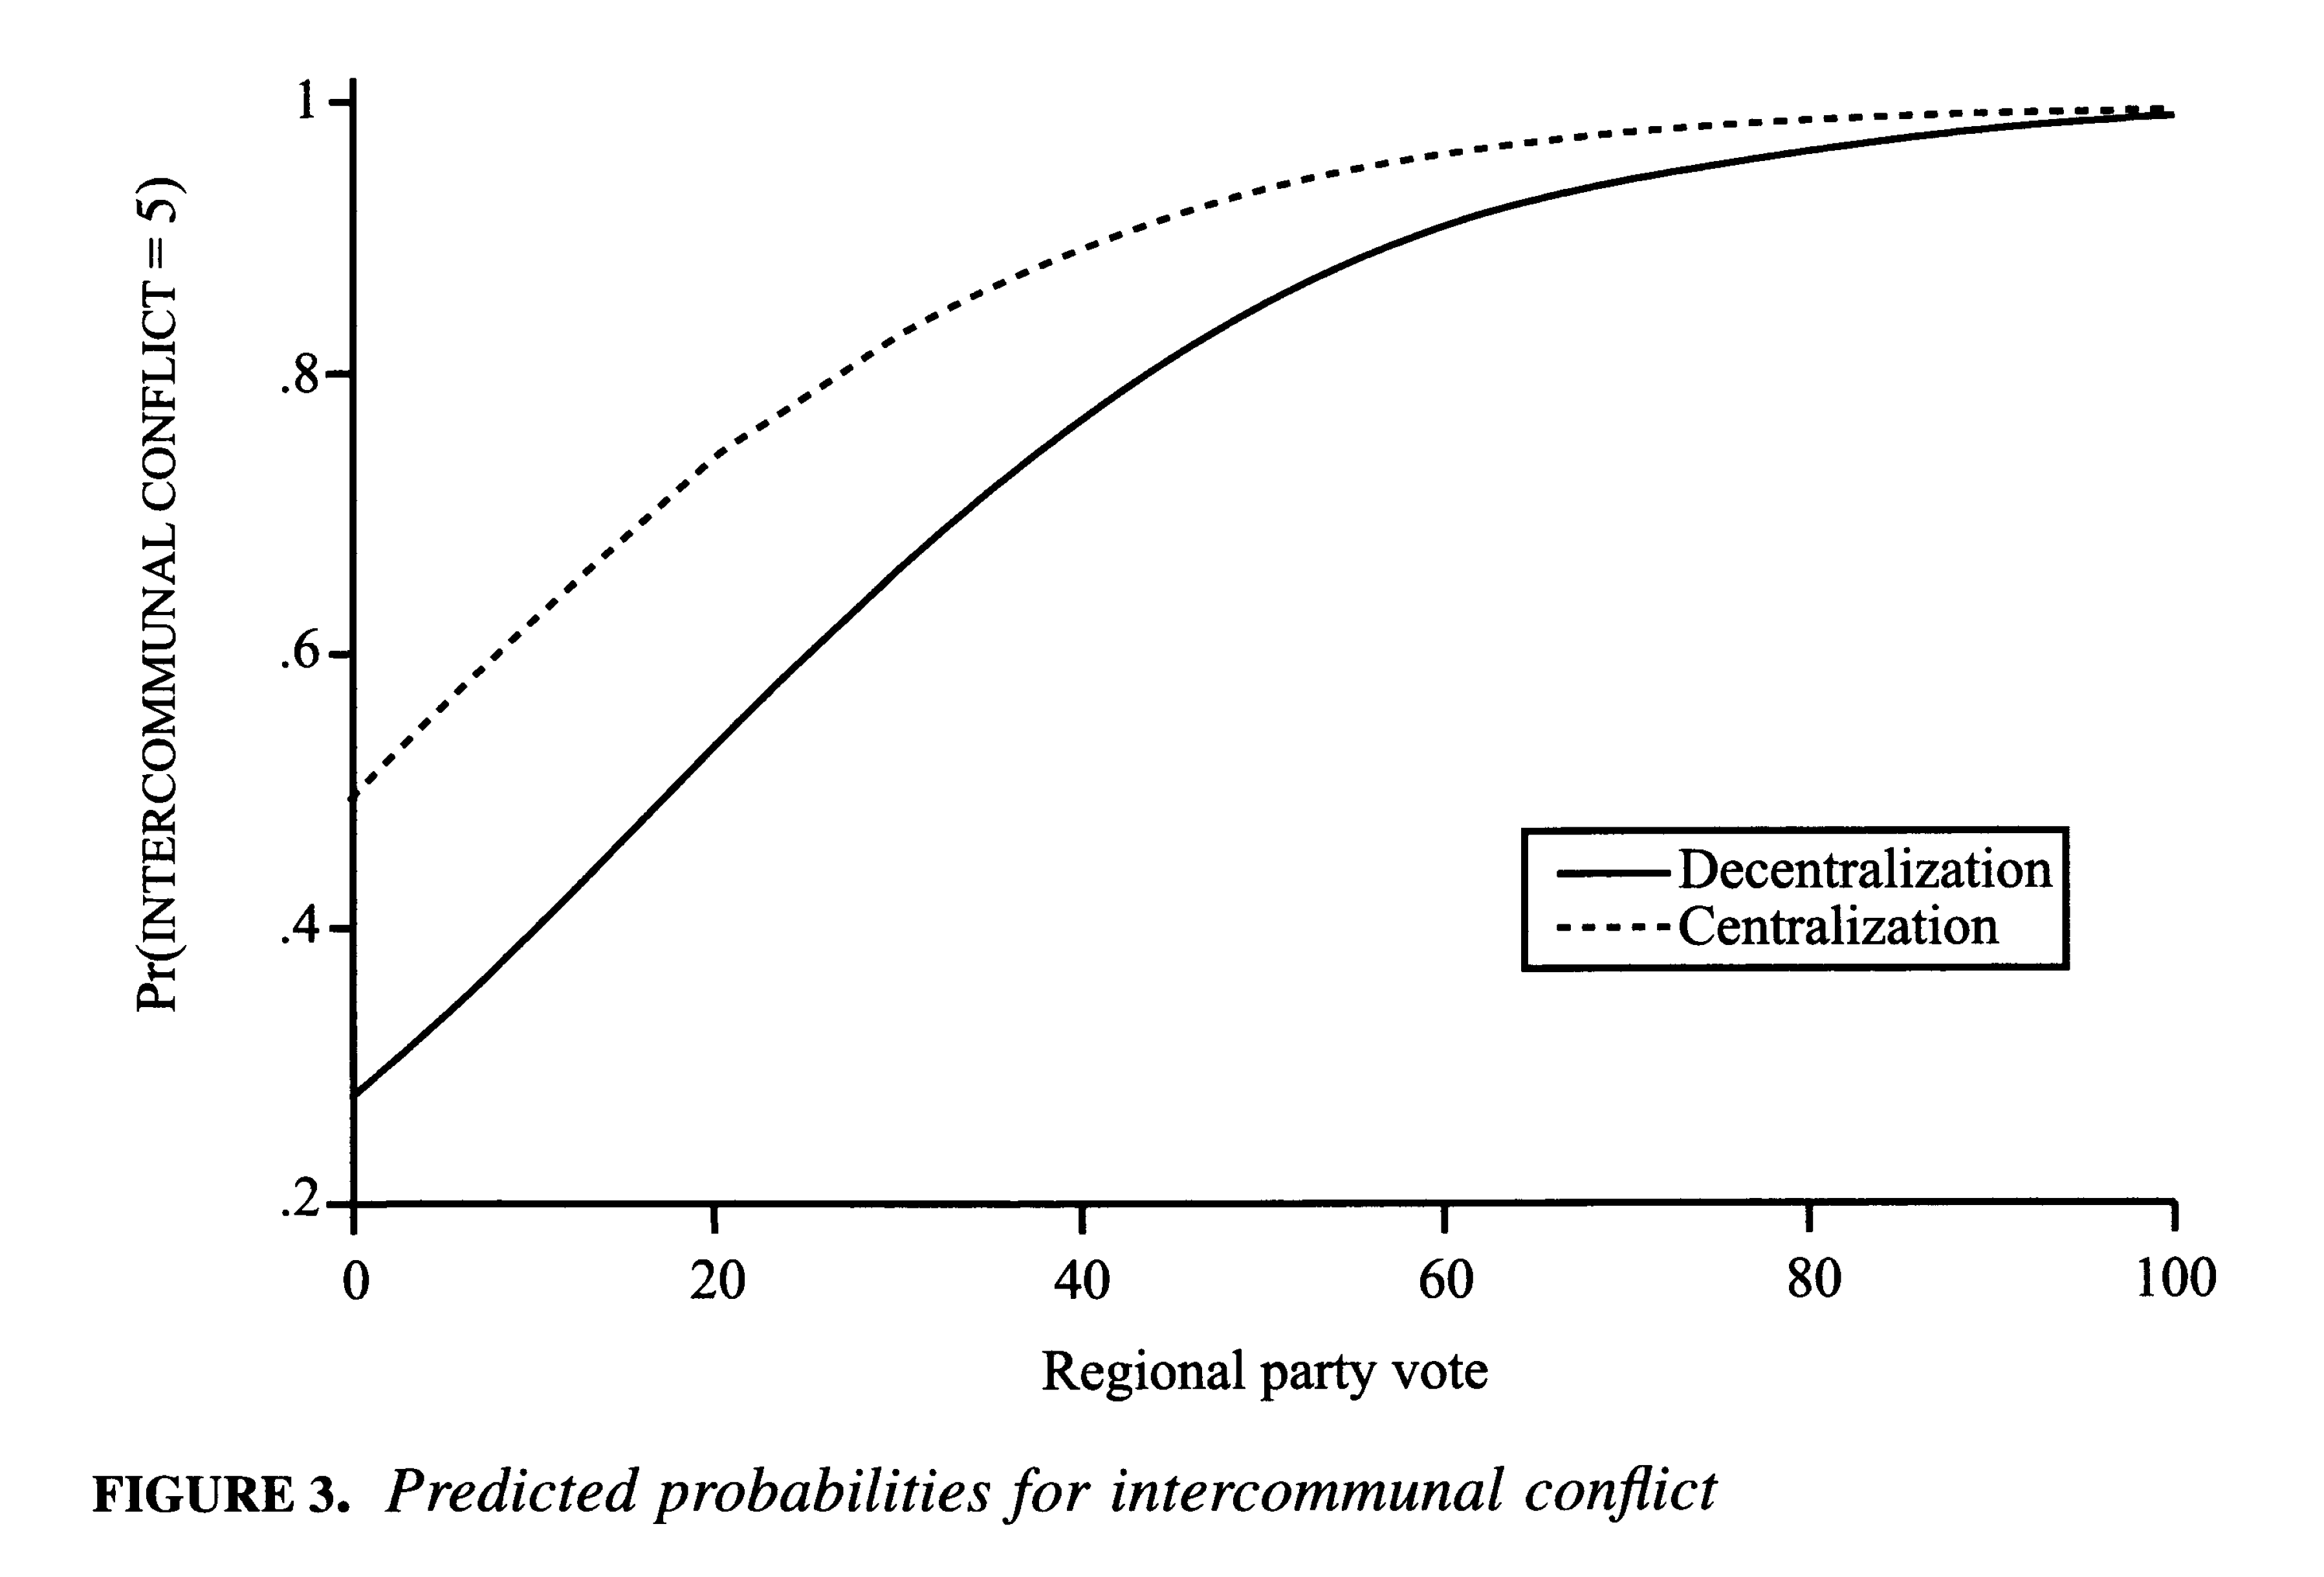
\includegraphics[width = \linewidth]{/Users/mz/Desktop/GitHub/teaching/gv217_conflict_analysis/figs/wk22/fig7.png}
    \end{center}
    \tiny © AFP/ Getty Images
\end{frame}

\begin{frame}{Women in Conflicts: Cases}
    \pause
    \begin{center}
        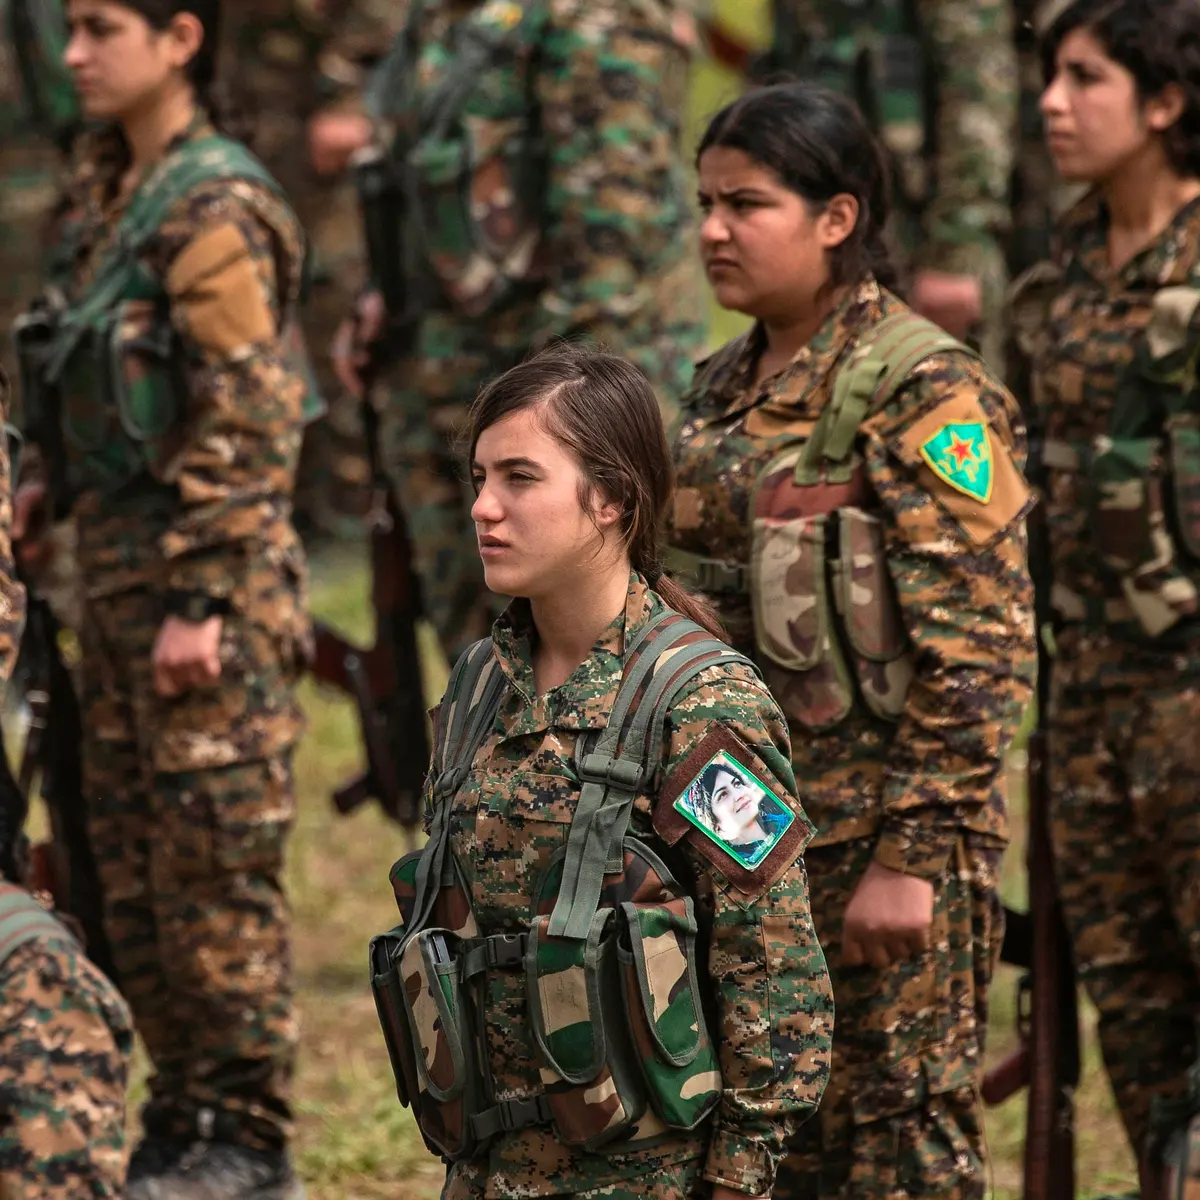
\includegraphics[width = \linewidth]{/Users/mz/Desktop/GitHub/teaching/gv217_conflict_analysis/figs/wk22/fig8.png}
    \end{center}
    \tiny \url{https://www.theguardian.com/global-development/2021/jul/19/came-to-fight-stayed-for-the-freedom-why-more-kurdish-women-are-taking-up-arms}
\end{frame}

\begin{frame}{Women in Conflicts: UNSC Resolution 1325 (2000)}
\begin{itemize}
    {\scriptsize
    \pause\item Expressing concern that civilians, particularly women and children, account for the vast majority of those adversely affected by armed conflict,
    \pause\item Reaffirming the important role of women in the prevention and resolution of conflicts and in peace-building,
    \pause\item Reaffirming also the need to implement fully international humanitarian and human rights law that protects the rights of women and girls during and after conflicts,
    \pause\item Emphasizing the need for all parties to ensure that mine clearance and mine awareness programmes take into account the special needs of women and girls,
    \pause\item Recognizing the urgent need to mainstream a gender perspective into peacekeeping operations,
    \pause\item Recognizing also the importance of the recommendation contained in the statement of its President to the press of 8 March 2000 for specialized training for all peacekeeping personnel on the protection, special needs and human rights of women and children in conflict situations,
    \pause\item Recognizing that an understanding of the impact of armed conflict on women and girls, effective institutional arrangements to guarantee their protection and full participation in the peace process can significantly contribute to the maintenance and promotion of international peace and security,
    \pause\item Noting the need to consolidate data on the impact of armed conflict on women and girls
    }
\end{itemize}
\end{frame}

\begin{frame}{Research Overview}
    \begin{itemize}
        \pause\item Women as victims
        \begin{itemize}
            \pause\item Sexual violence during conflicts
            \begin{itemize}
                \pause\item Why does it happen?
                \pause\item How does it afffect conflict (dynamics and outcomes)?
                \pause\item Reintegration and rehabilitation---how?
            \end{itemize}
            \pause\item Other types of gendered victimization
        \end{itemize}
        \pause\item Women as actors
        \begin{itemize}
            \pause\item Female combatants
            \begin{itemize}
                \pause\item Individual level: why do they join?
                \pause\item Upper level: what groups or conflicts have more?
                \pause\item How do they affect conflict?
                \pause\item Reintegration and rehabilitation---how?
            \end{itemize}
            \pause\item Female leaders
        \end{itemize}
    \end{itemize}
\end{frame}

\begin{frame}{Cohen (2009)}
    \begin{itemize}
        \pause\item Opportunism/greed
        \begin{itemize}
            \pause\item State collapse
            \pause\item Resources-abundance insurgency (why?)
        \end{itemize}
        \pause\item Gender inequality
        \pause\item Ethnic hatred
        \pause\item Forced recruitment (why?)
    \end{itemize}
\end{frame}

\begin{frame}{Wood \& Thomas (2017)}
    \pause The presence of a Marxist-oriented ``leftist'' ideology increases the prevalence of female fighters while Islamist ideologies exert the opposite effect.
\end{frame}

\begin{frame}{Wood \& Thomas (2017)}
    \pause \textit{Red Detachment of Women}
    \begin{center}
        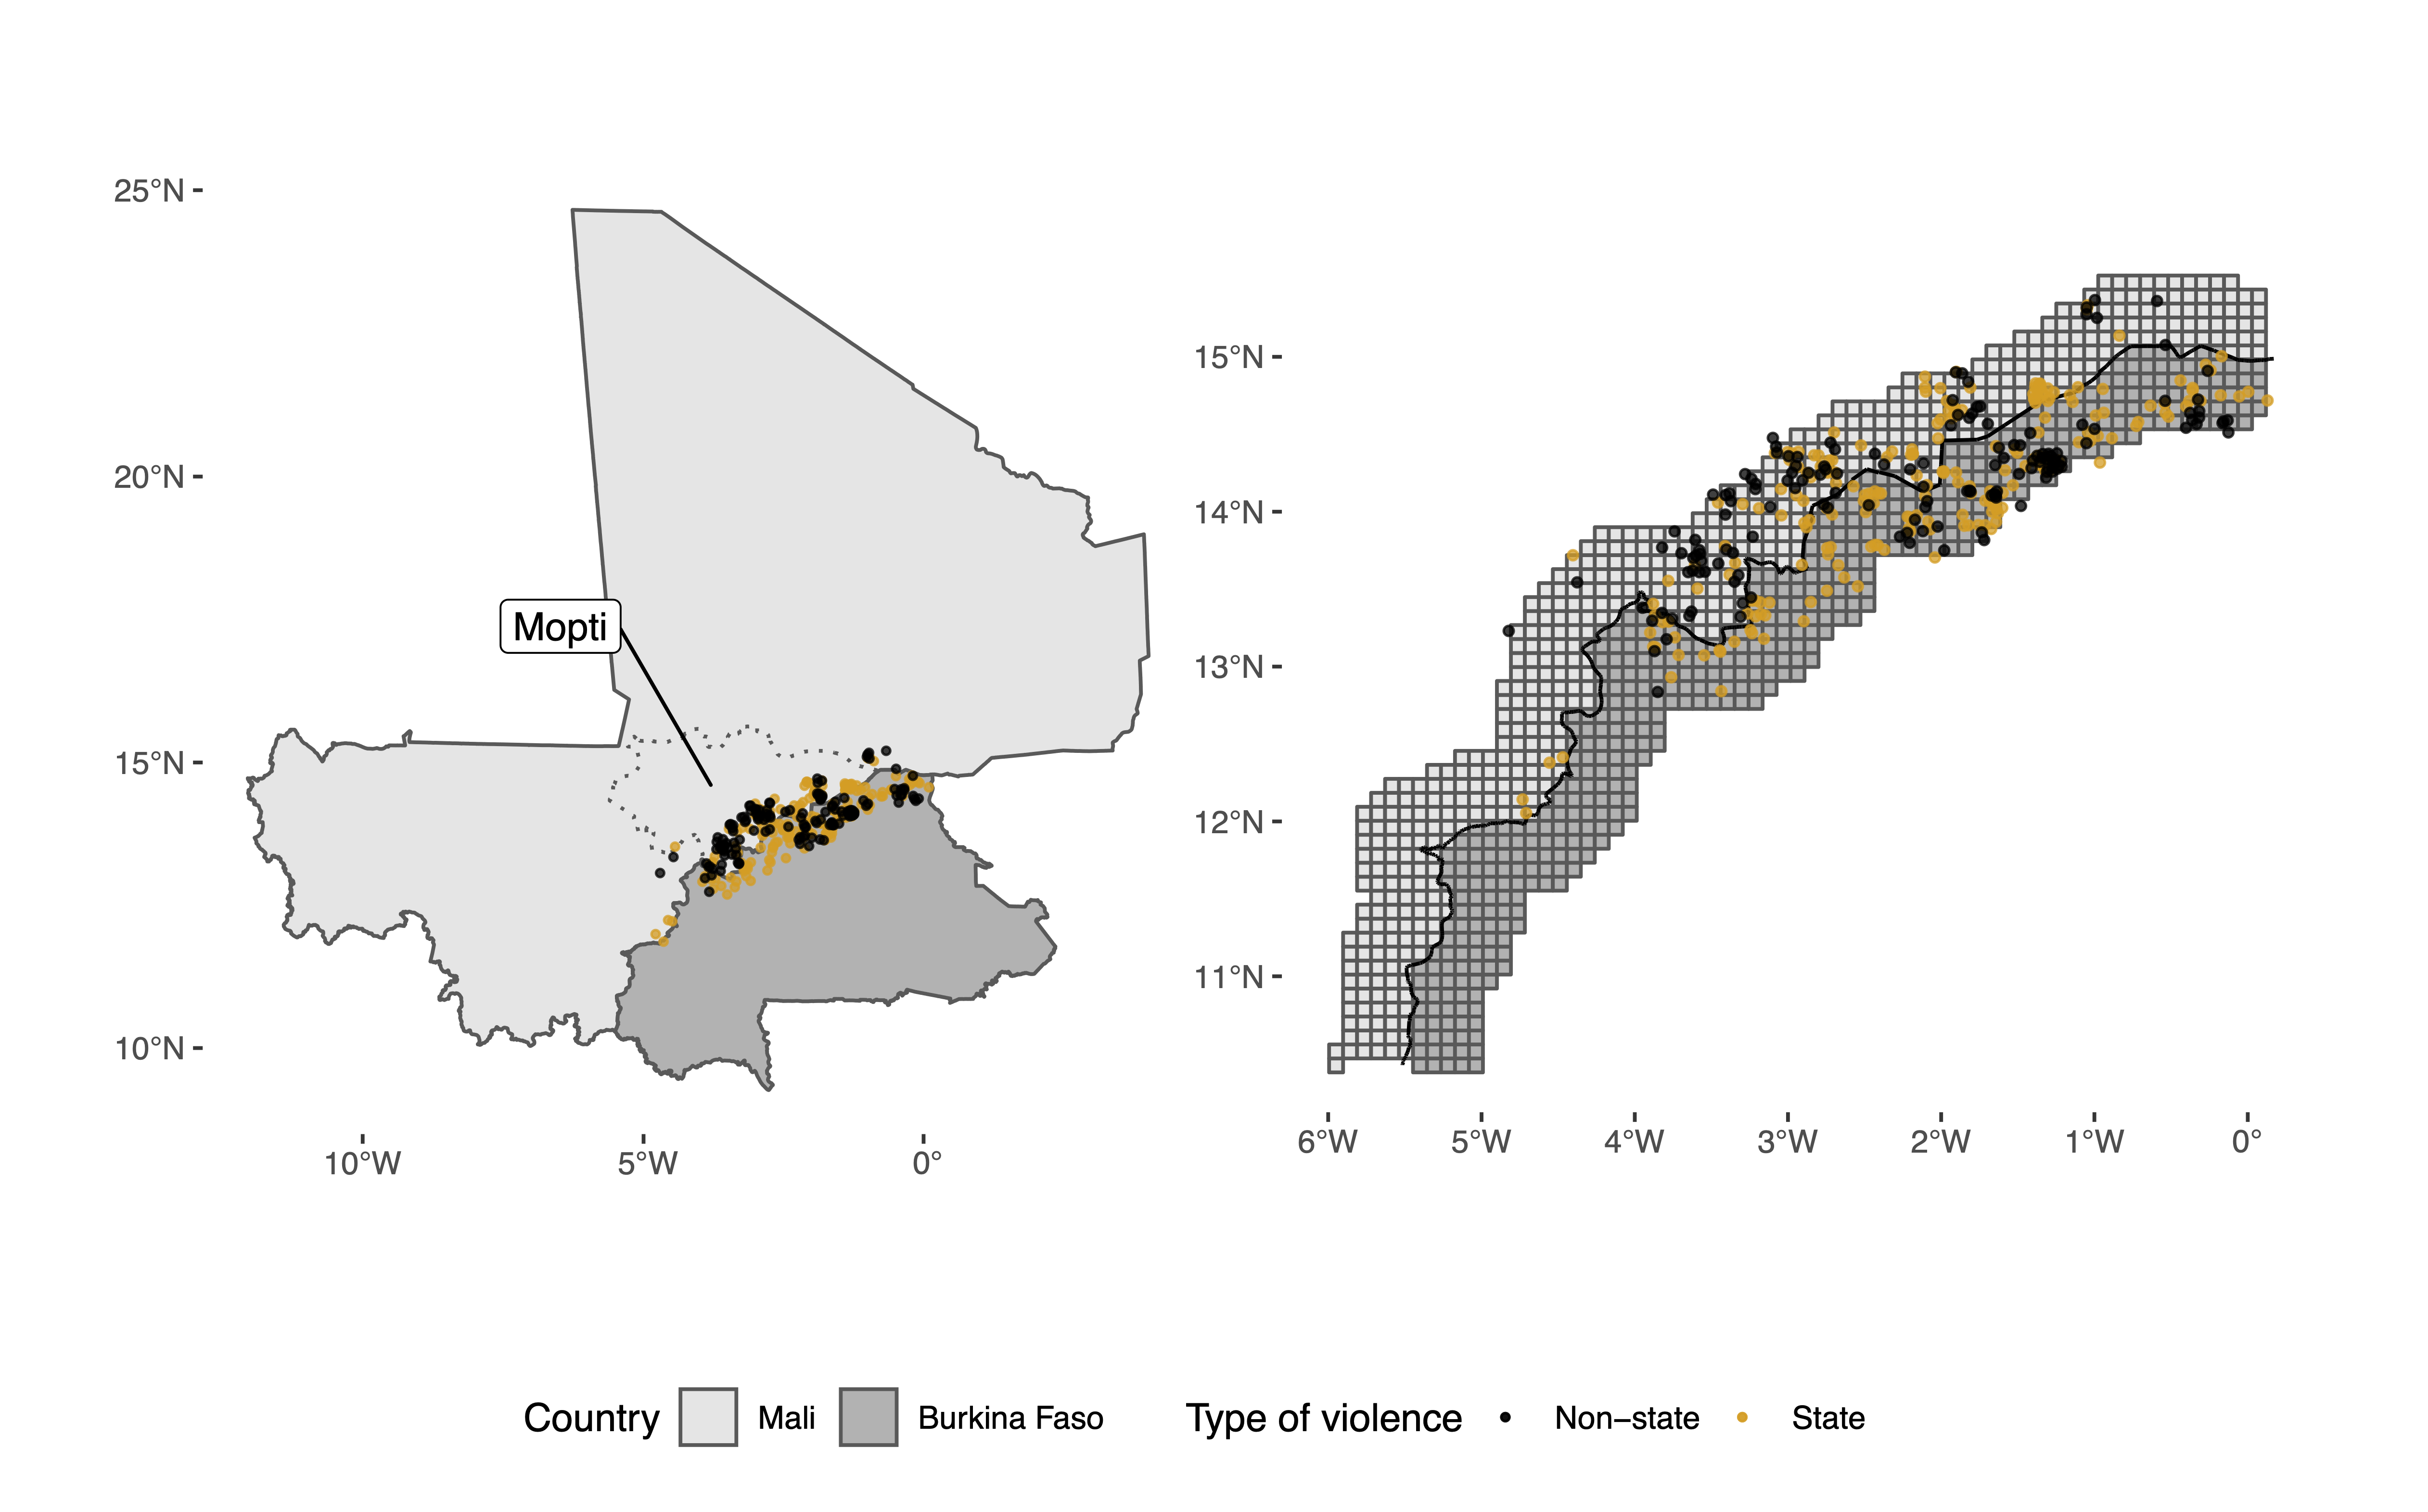
\includegraphics[width = \linewidth]{/Users/mz/Desktop/GitHub/teaching/gv217_conflict_analysis/figs/wk22/fig9.png}
    \end{center}
    \tiny \url{https://www.theguardian.com/global-development/2021/jul/19/came-to-fight-stayed-for-the-freedom-why-more-kurdish-women-are-taking-up-arms}
\end{frame}

\begin{frame}{Two More Questions}
    \begin{itemize}
        \pause\item Which previous argument relates to this week's?
        \pause\item Are the findings unbiased?\\
        \pause      Measurement error\\
        \pause      Conceptual \textit{versus} practical, LHS \textit{versus} RHS, random \textit{versus} non-random
    \end{itemize}
\end{frame}

\end{document}